\documentclass{cheatsheet}
\usepackage{bm}
\usepackage{textcomp, mathcomp}
\usepackage{empheq}
\usepackage{pbox}
\usepackage{booktabs}

\doctitle{Physik Zusammenfassung}
\author{Noa Sendlhofer \& Christian Leser \\ nsendlhofer \& cleser \\ \vspace*{-0.2em}}

\begin{document}
\section{1. Elektrizitätslehre}
    \subsection*{Basics}
    \begin{center}
        \textbf{Variablen}
        \begin{empheq}{align*} % Dipolmoment???
            \overrightarrow{B}                              &\quad \text{Magnetische Induktion}             & \scriptstyle T = \frac{W b}{m^2} = \frac{V \cdot s}{m^2} = \frac{kg}{A \cdot s^2} \\
            C                                               &\quad \text{Kapazität}                         & \scriptstyle F = \frac{C}{V} = \frac{A \cdot s}{V} = \frac{A^2 \cdot s^4}{kg \cdot m^2} \\
            D                                               &\quad \text{elek. Flussdichte /}               & \scriptstyle \frac{A \cdot s}{m^2}\\
                                                            &\quad \text{Verschiebungsdichte}               & \\
            \overrightarrow{E}                              &\quad \text{e. Feld}                           & \scriptstyle \frac{N}{C} = \frac{V}{m} = \frac{kg \cdot m}{s^3 \cdot A} \\
            E                                               &\quad \text{Energie} \quad 1eV \cdot e = 1J    & \scriptstyle J = Nm = CV = Ws \frac{kg \cdot m^2}{s^2} \\
            \scriptstyle f = \nu = \frac{1}{T}              &\quad \text{Frequenz}                          & \scriptstyle \frac{1}{s} = Hz \\
            \overrightarrow{F}                              &\quad \text{Kraft}                             & \scriptstyle N = \frac{V \cdot C}{m} = \frac{kg \cdot m}{s^2} \\
            \overrightarrow{H}                              &\quad \text{magn. Feldstärke}                  & \scriptstyle \frac{A}{m} \\
            \overrightarrow{I}                              &\quad \text{el. Strom}                         & \scriptstyle A = \frac{C}{s} \\
            \scriptstyle \overrightarrow{j} = \frac{I}{A}   &\quad \text{Stromdichte}                       & \scriptstyle \frac{C}{s \cdot m^2} \\
            k                                               &\quad \text{Federkonstante}                    & \scriptstyle \frac{N}{m} \\
            L                                               &\quad \text{Induktivität}                      & \scriptstyle H = \frac{T \cdot m^2}{A} = \frac{V \cdot s}{A} \\
                                                            &                                               & \scriptstyle = \frac{kg \cdot m^2}{A^2 \cdot s^2} \\
            P                                               &\quad \text{Leistung}                          & \scriptstyle W = V \cdot A = \frac{J}{s} \\
            Q                                               &\quad \text{Ladung}                            & \scriptstyle C = A \cdot s \\
            R                                               &\quad \text{el. Widerstand}                    & \scriptstyle \Omega = \frac{V}{A} \\
            S                                               &\quad \text{Siemens}                           & \scriptstyle S = \frac{1}{\Omega} = \frac{A}{V} \\
            T                                               &\quad \text{Periodendauer /}                   & \scriptstyle s \\
                                                            &\quad \text{Schwingungsdauer}                  & \\
            U                                               &\quad \text{Potentialdiff. / Spannung}         & \scriptstyle V = \frac{W}{A} = \frac{J}{C} \\
                                                            &                                               & \scriptstyle = \frac{Nm}{As} = \frac{kg \cdot m^2}{A \cdot s^3} \\
            \overrightarrow{v}                              &\quad \text{Geschwindigkeit}                   & \scriptstyle \frac{m}{s} \\
            W                                               &\quad \text{Arbeit}                            & \scriptstyle J = N \cdot m \\
                                                            &                                               & \scriptstyle = \frac{kg \cdot m^2}{s^2} = C \cdot V \\
            Z                                               &\quad \text{Impedanz}                          & \scriptstyle \Omega = \frac{V}{A} = \frac{kg \cdot m^2}{A^2 \cdot s^3} \\
            \varepsilon                                     &\quad \text{Dielektrizitätskonst. Mat.}        & \scriptstyle \frac{C}{V \cdot m} = \frac{A \cdot s}{V \cdot m} \\
            \Psi_E                                          &\quad \text{elek. Fluss}                       & \scriptstyle V \cdot m = \frac{N \cdot m^2}{C} \\
            \Phi_M                                          &\quad \text{magn. Fluss}                       & \scriptstyle Wb = T \cdot m^2 \\
            \Phi                                            &\quad \text{elek. Potential}                   & \scriptstyle [-] \\
            \lambda = \frac{c}{f}                           &\quad \text{Wellenlänge}                       & \scriptstyle m \\
            \mu                                             &\quad \text{magn. Feldk. /}                    & \scriptstyle \frac{V \cdot s}{A \cdot m} \\
                                                            &\quad \text{Permeabilität}                     & \\
            \rho                                            &\quad \text{spez. Widerstand}                  & \scriptstyle \Omega \cdot m \\
            \omega = 2 \pi f                                &\quad \text{Kreisfrequenz}                     & \scriptstyle s^{-1} = Hz \\
            %&\quad \text{} & \scriptstyle  \\
        \end{empheq}
        \textbf{Konstanten}
        \begin{empheq}{align*}
            g                                               &\quad \text{Fallbeschleunigung}                & \scriptstyle g \approx 9.81 \frac{m}{s^2} = \frac{N}{kg}\\
            \varepsilon_0                                   &\quad \text{el. Feldkonst /}                   & \scriptstyle \varepsilon_0 = \frac{1}{\mu_0 \cdot c_0^2} = \frac{10^7}{4 \pi c_0^2}\\
                                                            &\quad \text{Dielektrizitätskonst. /}           & \\
                                                            &\quad \text{Permittivität Vakuum}              & \\
            \varepsilon_{r, vak}                            &\quad \text{Permittivitätszahl Vakuum}         & \scriptstyle \varepsilon_{r, vak} = 1\\
            c_0                                             &\quad \text{Lichtgesch. Vakuum}                & \scriptstyle \frac{1}{\sqrt{\varepsilon_0 \mu_0}} \approx 3 \cdot 10^8 \frac{m}{s} \\
            \mu_0                                           &\quad \text{magn. Feldk. /}                    & \scriptstyle \mu_0 = \frac{1}{\varepsilon_0 c_0^2} = 4 \pi \cdot 10^{-7} \frac{V \cdot s}{A \cdot m} \\
                                                            &\quad \text{Permeabilität Vakuum}              & \\
            \mu_{r, vak}                                     &\quad \text{Permeabilitätszahl Vakuum}         & \scriptstyle \mu_{r, vak} = 1\\
            e                                               &\quad \text{Elementarladung}                   & \scriptstyle 1,602 \cdot 10^{-19} C \\
            m_e                                             &\quad \text{Elektronenmasse}                   & \scriptstyle = 9,11 \cdot 10^{-31} kg \\
            &\quad \text{} & \scriptstyle  \\
        \end{empheq}
        \textbf{Einheiten}
        \begin{empheq}{align*}
            eV                                              &\quad \text{Elektronenvolt (Energie)}          & \scriptstyle 1 e \cdot 1 V \\
            u                                               &\quad \text{Atomare Masseneinheit}             & \scriptstyle 1,66054 \cdot 10^{-27} kg \\
        \end{empheq}
        \textbf{Nutzliche Formeln}
        \begin{empheq}{align*}
            F_Z                                             &\quad \text{Zentripetalkraft}                  & \scriptstyle = m \frac{v^2}{r} = m \omega^2 r \\
            |\overrightarrow{a} \times \overrightarrow{b}|  &\quad \text{Kreuzprodukt}                      & \scriptstyle = |\overrightarrow{a}| \cdot |\overrightarrow{b}| \cdot \sin(\alpha)
        \end{empheq}
        \textbf{Maxwell-Gleichungen}
        \begin{enumerate}
            \item $\overrightarrow{\nabla} \cdot \overrightarrow{E} = \frac{\rho}{\varepsilon_0}$
            \item $\overrightarrow{\nabla} \cdot \overrightarrow{B} = 0$
            \item $\overrightarrow{\nabla} \times \overrightarrow{E} = -\frac{\partial \overrightarrow{B}}{\partial t}$
        \end{enumerate}
    \end{center}
    
    \begin{tabular}{c c c c c c c}
        \textbf{Symbol}     & P         & T         & G         & M         & k         & h   \\
        \textbf{Silbe}      & Peta      & Terra     & Giga      & Mega      & kilo      & hekto \\
        \textbf{Exponent}   & $10^{15}$ & $10^{12}$ & $10^9$    & $10^6$    & $10^3$    & $10^2$
    \end{tabular}
    \begin{tabular}{c c c c c c c c}
        d         & c         & m         & $\mu$         & n         & p           & f \\
        deci      & centi     & milli     & micro         & nano      & pico        & femto \\
        $10^{-1}$ & $10^{-2}$ & $10^{-3}$ & $10^{-6}$     & $10^{-9}$ & $10^{-12}$  & $10^{-15}$
    \end{tabular}
%        Y & $10^{24}$ \\
%        Z & $10^{21}$ \\
%        E & $10^{18}$ \\
%        da & $10^1$ \\
%        a & $10^{-18}$ \\
%        z & $10^{-21}$ \\
%        y & $10^{-24}$ 
    \subsection*{1.1 Definition Strom}

\begin{itemize}
    \item Ladungen mit gleichem Vorzeichen stossen sich ab.
    \item zwei unendlich lange parallele Drähte im Abstand 1 m voneinander, die von einem Strom von 1 A gleichsinnig durchflossen werden, ziehen sich mit einer Kraft von $2 \cdot 10^{-7} N$ pro Meter Leiterlänge an.
    \item Elementarladung: $e = 1.602 \cdot 10^{-19}$
\end{itemize}


Stromstärke: \mathbox{I = \frac{dQ}{dt}}
Ladung: \mathbox{Q = \int\limits_{\Delta t} I dt}
Widerstand: \mathbox{R = \frac{U}{I}, I \sim U}

\begin{tabular}{c c}
    Ohmsche Leiter & nicht-ohmsche Leiter \\
    $I = \frac{U}{R}$ & $R_{\text{diff}} = \frac{dU}{dI}$\\
    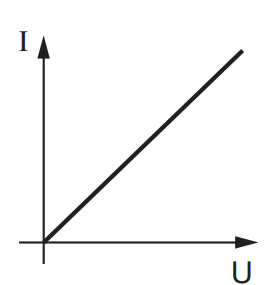
\includegraphics[width = 30mm]{src/images/plot_ohmscher_leiter.png} & 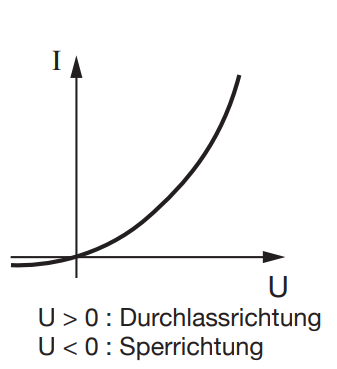
\includegraphics[width = 30mm]{src/images/plot_nicht-ohmscher_leiter.png}
\end{tabular}


    \subsection*{1.2 Klassifizierung ohmscher Leiter}
nach Grösse:
\mathbox{R = \rho \frac{l}{A}}, l Leiterlänge, A Leiterquerschnitt, $\rho$ spezifischer Widerstand
Spezifische Leitfähigkeit: $ K = \frac{1}{\rho}$\\
nach Temperatur:
\mathbox{\rho(T)}
    \subsection*{1.3 Kirchhoffsche Regeln}
    \subsubsection*{Knotenregel}
    \mathbox{\sum\limits_k I_k = 0}

    \subsubsection*{Maschenregel}
    \mathbox{\sum\limits_i U_i = \sum\limits_k I_k R_k}

    \subsubsection*{Serieschaltung}
    \[
        U_0 = I \cdot R_{tot} = I \cdot \left(\sum\limits_i R_i\right) \Rightarrow \boxed{R_{tot} = \sum\limits_i R_i}
    \]

    \subsubsection*{Parallelschaltung}
    \[
        I_{tot} = \frac{U}{R_{tot}} = \sum\limits_i \frac{U}{R_i} \Rightarrow \boxed{\frac{1}{R_{tot}} = \sum\limits_i \frac{1}{R_i}}
    \]

\section{2. Elektrisches Feld}

\section{3. Magnetisches Feld}

\section{4. Elektromagnetische Wellen}

\end{document}